\documentclass[11pt]{article}

\usepackage{ragged2e}
\justifying

\usepackage{helvet}
\renewcommand{\familydefault}{\sfdefault}
\usepackage[onehalfspacing]{setspace}

\usepackage[ngerman]{babel}

\usepackage{pifont}

\usepackage{microtype}
\usepackage{float}
\usepackage{hyperref}
\usepackage[margin=2.5cm]{geometry}
\usepackage{multirow,tabularx}
\newcolumntype{S}{>{\hsize=.75\hsize\arraybackslash}X}
\newcolumntype{N}{>{\hsize=1\hsize\arraybackslash}X}
\newcolumntype{B}{>{\hsize=1.5\hsize\arraybackslash}X}
\renewcommand{\arraystretch}{1}

\usepackage{verbatimbox}

\usepackage{xcolor}
\definecolor{bx-green}{HTML}{398772}
\usepackage{graphicx}
\graphicspath{{./pictures/}}
\usepackage{pdfpages}

\usepackage{fancyhdr}
\renewcommand{\headrule}{{\color{bx-green}\rule[2ex]{\dimexpr\textwidth-3.55cm}{.95pt}}}
\setlength{\headheight}{30pt}

\usepackage{sectsty}
\sectionfont{\color{bx-green}}  % sets colour of sections
\subsectionfont{\color{bx-green}}

\usepackage[utf8]{inputenc}
\usepackage[toc]{glossaries}
\usepackage[nottoc]{tocbibind}

\title{Beschte Onboarding}
\date{\today}
\author{Julian Thiele}


%---------------------------------------------------------------
%
%                   Listings
%
%---------------------------------------------------------------


\usepackage{listings}
\definecolor{lightgray}{rgb}{.9,.9,.9}
\definecolor{darkgray}{rgb}{.4,.4,.4}
\definecolor{purple}{rgb}{0.65, 0.12, 0.82}
\definecolor{darkgreen}{rgb}{0.02, 0.66, 0.23}
\lstdefinelanguage{TypeScript}{
    keywords={break, case, catch, continue, debugger, default, delete, do, else, false, finally, for, function, if, in, instanceof, new, null, return, switch, this, throw, true, try, typeof, var, void, while, with},
    morecomment=[l]{//},
    morecomment=[s]{/*}{*/},
    morestring=[b]',
    morestring=[b]",
    ndkeywords={class, export, boolean, throw, implements, import, this},
    keywordstyle=\color{blue}\bfseries,
    ndkeywordstyle=\color{darkgray}\bfseries,
    identifierstyle=\color{black},
    commentstyle=\color{purple}\ttfamily,
    stringstyle=\color{darkgreen}\ttfamily,
    sensitive=true
}

\lstset{
    language=TypeScript,
    backgroundcolor=\color{lightgray},
    extendedchars=true,
    basicstyle=\footnotesize\ttfamily,
    showstringspaces=false,
    showspaces=false,
    numbers=left,
    numberstyle=\footnotesize,
    numbersep=9pt,
    tabsize=2,
    breaklines=true,
    showtabs=false,
    captionpos=b
}
    
    
%---------------------------------------------------------------
%
%                   Glossar
%
%---------------------------------------------------------------
    
\makeglossaries
    
\newglossaryentry{vue}{
    name=vue,
    description={HTML-Framewok zum Erstellen von Webanwendungen}
}
\newglossaryentry{vscode}{
    name=VisualStudio Code,
    description={Code-Editor für die Programmierung von
    verschiedenen Programmiersprachen}
}
\newglossaryentry{firebase}{
    name=Firebase,
    description={Entwicklungsplattform für mobile und Webentwicklung, die
        Tools und Infrastruktur zur Verfügung stellt}
}
\newglossaryentry{firestore}{
    name=Firestore,
    description={NoSQL-Datenbank, die in Firebase integriert ist}
}
\newglossaryentry{NoSQL}{
    name=NoSQL,
    description={Nicht-relationale Datenbankstruktur ohne festgelegte Tabellenstruktue}
}
\newglossaryentry{git}{
    name=git,
    description={Software zur Versionsverwaltung von Dateien}
}
\newglossaryentry{buddy}{
    name=BREDEX-Buddy,
    description={Ansprechpartner für neue Mitarbeiter bei der BREDEX GmbH}
}
\newglossaryentry{achmnt}{
    name=Achievement,
    description={Aufgaben, die neue Mitarbeiter bei der BREDEX GmbH zusammen mit
    ihren BREDEX-Buddys erledigen können, um sich ins Unternehmen einzuarbeiten}
}
\newglossaryentry{modal}{
    name=modaldialog,
    description={Dialogfenster im Vordergrund einer Webanwendung}
}
\newglossaryentry{spa}{
    name=Single-Page Application,
    description={Eine Webanwendung, die aus einer einzigen HTML-Datei besteht, deren Inhalte dynamisch
        nachgeladen werden}
}
\newglossaryentry{api}{
    name=API,
    description={(Application Programming Interface / Programmierschnittstelle) Teil eines Softwaresytems,
        die dem Programmierer auf Quelltextebene den Anschluss an ein anderes System erlaubt}
}
\newglossaryentry{bt}{
    name=Bootstrap,
    description={CSS-Framework, das Gestaltungsvorlagen für Benutzeroberflächen bereitstellt}
}
\newglossaryentry{uuid}{
    name=UUID,
    description={(Universal Unique Identifier) 128-bit Zahl, die zur Identifikation von Informationen
        in Computersystemen genutzt wird}
}
\newglossaryentry{vuei18n}{
    name=Vue I18n,
    description={Vue Plugin, um leicht die Anwendung einer Sprache wechseln zu können}
}
\newglossaryentry{ref}{
    name=ref,
    description={Ein Objekt in Vue, dessen Wert in der Benutzeroberfläche in Echtzeit aktualisiert werden kann}
}
\newglossaryentry{baas}{
    name=Backend-As-A-Service,
    description={Dienst, der eine Entwicklungsumgebung im Browser zur Verfügung stellt mit Anbindung an eine Cloud,
        um die Entwicklung von Backends für Webanwendungen zu vereinfachen}
}
\newglossaryentry{unittest}{
    name=Unit-Tests,
    description={Automatisierte Tests, die Methoden auf korrekte Funktionsweise testen}
}
\newglossaryentry{expltest}{
    name=explorative Tests,
    description={Die Benutzeroberfläche wird von dem Testenden auf fehlerhafte oder falsche Eingaben überprüft,
        um Robustheit zu garantieren}
}
\newglossaryentry{usertest}{
    name=User-Test,
    description={Einen Nutzer werden Aufgaben gestellt, die dieser mit der Anwendung erledigen soll. Mit diesen Tests wird die
        intuitive Bedienbarkeit der Anwendung getestet}
}
\newglossaryentry{gamification}{
    name=Gamification,
    description={Übertragung von spieltypischen Elementen und Vorgängen in spielfremde Zusammenhänge}
}
\newglossaryentry{view}{
    name=view,
    description={Anderer Name für eine Komponente in Vue. Views sind in den meisten Fällen Komponenten, die eine Unterseiten der Webseite darstellen}
}
                    
                    
                    
%---------------------------------------------------------------
%
%                   BEGIN
%
%---------------------------------------------------------------
                    
                    
\begin{document}
\sloppy
       
\begin{titlepage}
    \vspace*{\fill}
        \centering
        {\Huge \textbf{Abschlussprüfung Winter 2023}\par}
        \vspace{1cm}
        {\Large \textbf{Ausbildungsberuf}\par}
        {\Large Fachinformatiker/Fachinformatikerin (VO 2020) \par Fachrichtung: Anwendungsentwicklung\par}
        \vspace{1cm}
        {\Large \textbf{Prüfungsbezirk}\par}
        {\Large Braunschweig 1201 FIA 4 (AP T2V1)\par}
        \vspace{1cm}
        {\Large \textbf{Prüfungsteilnehmer}\par}
        {\Large Herr Julian Thiele\par}
        {\Large Identnummer: 734117\par}
        \vspace{1cm}
        {\Large \textbf{Ausbildungsbetrieb}\par}
        {\Large Bredex GmbH\par}
        {\Large Lindentwete 1\par}
        {\Large 38100 Braunschweig\par}
        \vspace{1cm}
        {\Large \textbf{Projektbetreuer}\par}
        {\Large Herr Christian Rucinski\par}
        \vspace{1cm}
        {\Large \textbf{Thema der Projektarbeit}\par}
        {\Large Digitalisierung des internen Onboarding Prozesses neuer Mitarbeiter*innen\par}

    \vspace*{\fill}   
\end{titlepage}

% \maketitle
% \thispagestyle{empty}
% \newpage

\tableofcontents
\addtocontents{toc}{\protect\thispagestyle{empty}}
\pagenumbering{gobble}
\newpage
\pagenumbering{arabic}
\pagestyle{fancy}
\fancyhead[L]{Projektdokumentation - Julian Thiele}
\fancyhead[R]{
    \vspace*{-.4cm}
    
\includegraphics[height=.7cm]{bx_logo.png}
}
                    
%---------------------------------------------------------------
%
%                   INTRODUCTION
%
%---------------------------------------------------------------
                    
\section{Einleitung}
                    
\subsection{Ausbildungsbetrieb}
Die BREDEX GmbH wurde im Jahr 1987 in Braunschweig gegründet. Den Schwerpunkt 
bildet die individuelle Softwareentwicklung, BREDEX führt jedoch auch 
Beratungen zu Datenschutz, Datensicherheit, Qualitätssicherung von Software 
und Schulungen durch. Die BREDEX GmbH besitzt, mit ihrer Tochterfirma BREDEX 
HUNGARY KFT. zusammen, ca. 200 Mitarbeiter. Davon sind ungefähr 12 Mitarbeiter Auszubildenden und dualen Studenten.  % Azubis / Dualis?

\subsection{Projektumfeld}
Das Projekt wird unter der Aufsicht von Herr Christian Rucinski in den 
Geschäftsräumen der BREDEX GmbH entwickelt. Bei der Anwendung handelt es sich 
um ein BREDEX internes Tool. Sie soll für den Onboardingprozess neuer Mitarbeiter 
eingesetzt werden und den sogenannten \Gls{buddy}, einen Ansprechpartner 
neuer Mitarbeiter, bei seiner Arbeit unterstützen. 

Das Frontend wird mit dem Framework \Gls{vue}, bei welchem die Scriptsprache TypeScript 
Anwendung findet, geschrieben. Als Backend wird \gls{firebase} als “Backend As a Service” 
genutzt, in welche die NoSQL-Datenbank \gls{firestore} integriert ist.

\subsection{Projektabgrenzung}
Durch die Fachinformatikerausbildungsverordung wird das Projekt zeitlich auf 80 
Stunden begrenzt.  

Die Anwendung ist ein alleinstehendes Tool und wird daher in kein Projekt 
eingegliedert. Daher gibt es keine weiteren Beschränkungen, auf die geachtet 
werden muss.  

\subsection{Projektziel}
Um neuen Mitarbeitern den Start in das Unternehmen zu vereinfachen, stellt BREDEX GmbH neuen Mitarbeitern
den sogenannten \gls{buddy} zur Verfügung. Um diesen in Zukunft die Arbeit zu vereinfachen und ihnen die Aufgaben klarzustellen,
soll es in Zukunft eine Webanwendung geben. Diese soll eine Checkliste mit den verschiedenen Aufgaben zur Verfügung stellen, die ein
\Gls{buddy} erledigen soll, sowie eine Rangliste, um die Einarbeitung mithilfe von \Gls{gamification} interessanter zu gestalten.

\subsection{Abweichungen vom Projektantrag}
Es gibt keine Abweichungen vom Projektantrag.

\subsection{weitere Anmerkungen}
In der Dokumentation wird die männliche Form von Mitarbeitern, Kollegen, Kunden, etc genutzt.
Gemeint wird jedoch m/w/d.


%---------------------------------------------------------------
%
%                   Projektplanung
%
%---------------------------------------------------------------

\section{Projektplanung}
Bei der Projektplanung werden die benötigten Arbeitspakete identifiziert und geplant.
Zudem werden Kosten und Ressourcen zunächst abgeschätzt.

\subsection{Identifizierung der Arbeitspakete}
Zu Beginn fand ein Anforderungsgespräch statt. Hierbei wurden die Projektziele 
definiert, damit es keine Differenzen im Verständnis dieser gibt. Außerden wurde definiert, welche Anforderungen erfüllt werden müssen. 

Im Anschluss folgte die Analysephase. In dieser Phase wurde der IST-Zustand analysiert und 
der Soll-Zustand niedergeschrieben, welcher sich aus den vorab definierten Anforderungen ergab.
Dabei wurden die Anforderungen verfeinert.

Auf den Verfeinerungen der Analysephase baute die folgende Designphase auf.
Hierbei wurde die Benutzeroberfläche geplant und
ein Datenmodell erstellt. Dadurch konnten benötigte Ressourcen genauer abgeschätzt werden.

Daraufhin folgte die Entwicklung der Anwendung, bei der die Ergebnisse der 
vorherigen Arbeitspaketen umgesetzt wurden. Um mögliche Fehler während der 
Implementierung frühzeitig erkennen und beheben zu können, fanden Tests statt. 

Am Ende der Entwicklungsphase wurde ein Abnahmegespräch mit dem Projektbetreuer durchgeführt. 
In diesem Gespräch wurde die Anwendung mit den Anforderungen verglichen und entschieden, ob diese
erfüllt wurden.

Im letzten Arbeitsschritt wurde die Dokumentation des Projektes erstellt. 

\subsection{Zeitplan}
Das vorliegende Projekt wurde im Zeitraum vom 22.09.2023 bis zum 22.11.2023 bearbeitet. 
Für die unter 2.1 genannten Arbeitspakete wurde folgend der Zeitplan 
(\autoref{table:timeplan}) erstellt. 

\begin{table}[H]
    \centering
    \begin{tabular}{|l | l|}
        \hline
        Arbeitspaket & Dauer \\
        & (in Stunden) \\
        \hline
        Anforderungsgespräch & 3 \\
        Analysephase & 6 \\
        Planungsphase & 6 \\
        Designphase & 6 \\
        Umsetzung & 40 \\
        Test und Abnahme & 7 \\
        Dokumentation & 12 \\
        \hline
        \textbf{Gesamt} & \textbf{80} \\
        \hline
    \end{tabular}
    \caption{Zeitplan}
    \label{table:timeplan}
\end{table}

\subsection{Ressourcenplanung}
Um die Kosten so gering wie möglich zu halten, wurde nach Möglichkeit nur
kostenlose oder bereits vorhandene Software, sowie Hardware genutzt.
Als Arbeitsgerät wurde durch die BREDEX GmbH ein Laptop mit Windows 10 und der
Entwicklungsumgebung \gls{vscode} bereitgestellt.
Des Weiteren wurde \gls{firebase} als \gls*{baas} mit \gls{firestore} als Datenbank verwendet. \Gls{git} wird als 
Versionsverwaltung eingesetzt.\newline
Eine Liste mit allen genutzten Ressourcen befindet sich im Anhang. 

\subsection{Kostenplanung}
Für den Prüfungsteilnehmer wurde ein Stundenlohn von 9 EUR angesetzt. % Mischkalkulation ?
Ihm standen für die Bearbeitung 80 Stunden zur Verfügung.
Der Projektbetreuer führte das Anforderungsgespräch durch und stand 
dazu noch für weitere Fragen während der Bearbeitung zur Verfügung.
Daher wurden für ihn 6 Stunden angesetzt, bei einem geschätzten 
Stundenlohn von 45 EUR.
Da ansonsten nur vorhandene oder kostenlose Ressourcen genutzt wurden,
ergaben sich keine weiteren Lizenz- oder Nutzungskosten.

Als Gesamtkosten ergaben sich hiermit 990 EUR, wie im Kostenplan (s. \autoref{table:costs}) festgehlaten.




\subsection{Nutzwertanalyse}

Das Ziel der Anwendung liegt darin, den Prozess der Einarbeitung neuer Mitarbeiter zu erleichtern. Unter diesem Gesichtspunkt wird im Folgenden der alte Prozess
mit dem neuen Prozess, der die hier entwickelte Anwendung nutzt, verglichen. Die Nutzwerte wurden ermittelt und im Anhang in \autoref{table:weightedsum} festgehalten.

Am Wichtigsten ist der Aspekt der Benutzerfreundlichkeit (Usability). Im alten Prozess mussten alle Aufgaben per Hand aus einer Word-Datei in eine eigene
Liste kopiert werden und bei Erfüllung manuell durch Emojis abgehakt oder aus der eigenen Liste gelöscht werden. 
Außerdem mussten alle Aufgaben für nicht-deutschsprachige Mitarbeiter vom \Gls{buddy} selbst übersetzt werden.\newline
In der Anwendung werden die Aufgaben über die \glspl{achmnt} direkt in einer Liste gesammelt und können durch einen einfachen Klick abgehakt werden.
Die Sprache kann über einen Button in der Anwendung einfach umgestellt werden.

Ein weiterer Wert der Anwendung liegt in der Vereinheitlichung des Prozesses. Derzeit gibt es unterschiedliche Listen mit verschiedenen Aufgaben. Je nachdem, welche Liste der
\Gls{buddy} nutzt, werden unterschiedliche Aufgaben erledigt. \newline
Mit der Anwendung gibt es eine einheitliche Liste an \glspl{achmnt}, die von den \Glspl{buddy} genutzt wird. Diese Liste kann jederzeit von 
zuständigen Personen angepasst werden, sollte es Änderungen im Einarbeitungsprozess geben.

Die Motivation die Aufgaben zu erledigen steigt vorraussichtlich mit der Anwendung deutlich an. Der Vorgang, die Aufgaben zu suchen, und alles manuell kopieren
zu müssen ist umständlich, was die Motivation senkt, sich darum zu kümmern. Mit der Anwendung müssen die Aufgaben nicht mehr gesucht werden, sondern
sind einfach in der Applikation einsehbar. Außerdem erhält die Einarbeitung durch die Rangliste eine \Gls{gamification}. Dadurch kann die Motivation weiterhin gesteigert werden, 
da man sich mit seinen Kollegen messen kann und ein kleiner Wettbewerb entsteht.

Schließlich wird der Aspekt der Sicherheit betrachtet. Die alten Dateien an Aufgaben lagen in einem zentralen Cloudspeicher und konnten von allen Mitarbeitern bearbeitet
oder neu erstellt werden. Mit der neuen Anwendung können nur noch zuständige Personen auf die Liste zugreifen, um diese zu bearbeiten.  



%---------------------------------------------------------------
%
%                   Analysephase
%
%---------------------------------------------------------------

\section{Analysephase}
In der Analysephase werden die Anforderungen definiert, sowie der IST-Zustand analysiert und das
SOLL-Konzept entwickelt. Mit den Erkenntnissen aus dieser Phase kann im Anschluss die Struktur
der Anwendung erstellt werden.

\subsection{Anforderungsgespräch}
Als Erstes wurde ein Anforderungsgespräch mit dem Kunden durchgeführt.
In dem Gespräch wird der IST-Zustand ermittelt und das SOLL-Konzept definiert.
Außerdem wurden die vom Kunden gewünschten Features der Amwendung übermittelt.
Die wichtigsten Features der Anwendung sind:

\begin{itemize} 
    \item \glspl{achmnt}, die abgehakt werden können
    \item Rangliste, um sich mit Kollegen vergleichen zu können
    \item Als Administrator Achievementliste bearbeiten können 
    \item Mehrsprachigkeit in Deutsch und Englisch
\end{itemize}

Die Punkte wurden in dem Gespräch noch weiter konkretisiert, um die Anwendung
im Anschluss möglichst nach den Wünschen des Kunden implementieren zu können.


\subsection{IST-Zustand Analyse}

Damit neue Mitarbeiter der BREDEX GmbH besser in das Unternehmen
finden, wird ihnen ein Ansprechpartner, der sogenannte \gls{buddy},
an die Seite gestellt. Dieser soll dem Mitarbeiter das Unternehmen
näherbringen. Allerdings ist nicht genau klar, was die Aufgaben des \Glspl{buddy}
beinhalten. Es gibt unterschiedliche Orte, an denen man Listen mit
verschiedenen Inhalten findet. 
Dadurch führen die \Glspl{buddy} ihre Aufgabe unterschiedlich aus. Daraus resultiert, 
dass Mitarbeiter unterschiedlich eingearbeitet werden und es besteht die
Möglichkeit, dass Punkte vergessen oder vernachlässigt werden. Dadurch erfahren neue Mitarbeiter beispielsweise nicht
von Angeboten, die die BREDEX GmbH zur Verfügung stellt, bekommen Ereignisse nicht mit oder lernen ihre Kollegen nicht kennen,
weshalb sie sich schwerer in das Unternehmen einfinden, wodurch auch die Produktivität leiden kann. \newline % Problem? -d
Zudem ist der Prozess sehr umständlich. Die Aufgaben müssen aus der Datei in eine eigene kopiert werden,
um sie abhaken zu können. Das Abhaken der erledigten Aufgaben erfolgt händisch über Löschen der Einträge, 
Einfügen eines Haken-Emojis oder Ähnlichem. 


\subsection{SOLL-Konzept}

Um in Zukunft dafür zu sorgen, dass alle \Glspl{buddy} ihre Aufgaben auf die gleiche Art
und Weise erledigen und den Prozess im Allgemeinen zu vereinfachen, soll eine Webanwendung programmiert werden. 
In der Anwendung soll es eine Checkliste an \glspl{achmnt} geben, die neue Mitarbeiter im Verlauf ihrer Einarbeitung
mit ihren \Glspl{buddy} zusammen abarbeiten können. Diese Achievements sollen verschiedene Aufgaben beinhalten, wie beispielsweise bestimmte
Personen aus dem Unternehmen kennen zu lernen oder sich über Angebote oder Abläufe zu informieren. Manche Achievements beinhalten zudem
Referenzen zu Insidern aus der Unternehmenskultur, wodurch man diese besser kennen lernt.

Zudem soll es eine Rangliste geben, in der sich Kollegen, die zur selben Zeit angefangen haben, gegenseitig
sehen können. Diese \Gls{gamification} erhöht die Motivation, \glspl{achmnt} zu erledigen. Dadurch lernen neue Mitarbeiter
das Unternehmen schneller kennen und finden sich so schneller zurecht und lernen ihre Kollegen schneller kennen. 

Um die \glspl{achmnt} aktualisieren zu können, soll es noch eine Seite geben, bei der ausgewählte
Personen neue \glspl{achmnt} anlegen, bearbeiten oder auch löschen können. Dadurch können die Achievements besser aktuell gehalten werden und bei
Änderungen im Unternehmen oder anderem Bedarf angepasst werden. Hierbei müssen beide Sprachen von den Nutzern gepflegt werden.
Nicht autorisierte Personen sollen diese Seite weder sehen, noch darauf zugreifen können.


%---------------------------------------------------------------
%
%                   Design
%
%---------------------------------------------------------------

\section{Designphase}
In der Designphase werden Benutzeroberfläche und Datenmodelle der Anwendung geplant. Dadurch können benötigte Ressourcen
genauer abgeschätzt sowie Schwierigkeiten oder Fehler im Vorraus erkannt werden. 

\subsection{Benutzeroberfläche}

% Corporate Design - BX style guide
% standard Login-Seite

Bei dem Design der Benutzeroberfläche (im folgenden GUI genannt) wird
besonders darauf geachtet, dass alle Daten möglichst übersichtlich
dargestellt werden. Dazu werden für jede der großen Anforderungen
jeweils einzelne Unterseiten (im folgenden \Gls{view} genannt) unterteilt. 

Hierbei gibt es eine \Gls{view}, um alle \glspl{achmnt} einsehen
und abhaken zu können. \Glspl{achmnt} werden zu verschiedenen
Zeitpunkten freigeschaltet. Manche sind direkt verfügbar, manche 
nach einer Woche, einem Monat oder erst nach einem halben Jahr. 
Entsprechend dieser Zeitstempel sind die \glspl{achmnt} in Akkordeons
gruppiert. Dies führt dazu, dass \glspl{achmnt} übersichtlich einsehbar
sind.

Eine weitere \Gls{view} gibt es für die Ansicht der Rangliste. Hier wird
der derzeit eingeloggten Person eine Rangliste mit den Personen, die
zu einer ähnlichen Zeit angefangen haben, angezeigt. Jeder wird mit Platzierung,
Punktzahl, Name, sowie der Email-Adresse angezeigt (\autoref{abb:ranking}).

Eine letzte \Gls{view} dient der Verwaltung von \Glspl{achmnt}.
Die \Gls{view} ist ähnlich aufgebaut, wie die \glspl{achmnt}-\Gls{view}. Neben den Akkordeon-Headern befindet sich
zusätzlich jeweils ein weiterer Button, um neue \glspl{achmnt} für diesen Zeitpunkt
hinzufügen zu können. Anstatt \glspl{achmnt} abzuhaken zu können, findet der Nutzer hier
einen Button, um \glspl{achmnt} zu bearbeiten oder zu löschen (\autoref{abb:achievements_manage}).

Beim Hinzufügen oder Bearbeiten eines \glspl{achmnt} öffnet sich ein
\Gls{modal}. Ín diesem Dialogfenster kann der deutsche und englische Text, sowie der
Zeitpunkt für die Freischaltung des Achievements und die Punktzahl eingestellt werden (\autoref{abb:modal}). 
Bei Bstätigung des Dialoges werden die Daten in die Datenbak übertragen und dort gespeichert.
Fehlende Eingaben werden dem Nutzer über eine Eingabeaufforderung am jeweiligen Eingabefeld gekennzeichnet.

Um ein einheitliches Design mit anderen internen Applikationen der BREDEX GmbH herzustellen, wurde der Stil der Software
am BREDEX-Styleguide orientiert. Hier sind grundsätzliche Designentscheidungen für BREDEX-Software, wie z.B. Farben oder Schrift normiert.
Auch die Login-Seite ist dem standardisierten Design der BREDEX GmbH angepasst.

\subsection{Datenbank}

Bei der Datenbank handelt es sich um die \gls{NoSQL}-Datenbank \gls{firebase}
von \gls{firestore}. Die Daten werden im JSON-Format gespeichert. Hierbei wird
von Sammlungen und Attributen gesprochen. Sammlungen sind mehrere JSON-Objekte, mit einer
ID und einem Datensatz. Dieser Datensatz kann weitere Sammlungen beinhalten,
sowie Attribute wie beispielsweise Zahlen, Zeichenketten oder Arrays.

Um die \glspl{achmnt} und die Daten der Nutzer der Anwendung speichern zu können,
wurden in der Datenbank jeweils Sammlungen angelegt. Die Referenzen der Nutzer zu ihren
erledigten Achievements werden in einer ID-Liste gespeichert, anstatt eine Benutzereigene Sammlung für Achievements
anzulegen. Dies entspricht eher einem relationalen Ansatz, der eher unüblich für \Gls{NoSQL}-Datenbanken ist.
Die Entscheidung wurde getroffen, um die Redundanz von Daten zu verringern und das Pflegen von Achievements
einfacher Umsetzen zu können. 
% hiervor könntest du noch dediziert schreiben wofür eine Sammlung steht. Das wird hier nicht klar -- jetzt klar?


%---------------------------------------------------------------
%
%                   Implementierung
%
%---------------------------------------------------------------

\section{Implementierungsphase}
In der Implementierungsphase wird die Anwendung programmiert. Hierbei werden die,
in der Planungs- und Designphase erstellten, Strukturen und Modelle genutzt, um die Software möglichst ohne
Komplikationen umsetzen zu können.

\subsection{Frontend}

% installation

Im Frontend wird das Webframework \Gls{vue} eingesetzt. Dieses baut auf den
standard Websprachen HTML, JavaScript und CSS auf. 
\Gls{vue} nutzt komponentenbasierte Programmierung, indem es HTML um die Möglichkeit
erweitert, Templates zu erzeugen. Durch diese Templates wird dann, entsprechend dem zugrunde 
liegenden Java-Scripts, die GUI erzeugt. % Erklärung besser ?
In dieser Anwendung wird Vue-Routing genutzt, um eine \gls{spa} zu
erstellen. Die Webseite besteht bei einer \gls{spa} nur aus einer HTML-Datei. Diese Datei
wird von \Gls{vue} im Buildprozess der Anwendung erstellt. Der Inhalt des HTML kann dynamisch mit den
verschidenen Komponenten ausgetauscht werden.

Standardmäßig wird in \Gls{vue} die Scriptsprache JavaScript genutzt. Das Framework
kann auch mit der Sprache TypeScript genutzt werden, wofür sich in diesem
Projekt entschieden wurde, um die Vorteile von Typisierung nutzen zu können.
Dadurch können gewisse Fehler bereits zur Kompilierzeit vom Compiler entdeckt werden und
die Anwendung gegenüber Fehlern robsuter gemacht werden.

\Gls{vue} stellt seit Version 3.0 auch eine neue \gls{api} zur Verfügung: die Composition \Gls{api}.
Die Vorteile gegenüber der, in \Gls{vue} standardmäßig genutzten, Options \Gls{api}, ist die Möglichkeit,
den Code variabler und besser strukturieren zu können. Dies verbessert die Lesbarkeit und Qualität des
Codes. Außerdem erleichtert die Composition \Gls{api} die Wiederverwendbarkeit
von Code in verschiedenen Komponenten, was eine große Auswirkung auf Codequalität und
Fehlerrobustheit hat.

Für Styling wird das CSS-Framework \gls{bt} genutzt, um einfacher ein modernes
Design für die Anwendung erstellen zu können und sich auf die Programmierung des
Projektes konzentrieren zu können.\newline

% Zu detailliert / Überflüssig?
% View organisiert die Website über mehrere Single-Page-Komponenten. Hierbei handelt
% es sich um eine Dateistruktur, bei der jede Datei seine eigene Komponente beinhält.
% Die Wurzelkomponente einer jeden Vue-Amwemdung stellt die App-Component dar. In dieser
% wird der <vue-router> Tag genutzt. Dadurch lässt sich ein Teil des Inhaltes der App-Komponente
% dynamisch mit anderen Komponenten austauschen. % Header mit v-if

Als erstes wurde die Achievement-\Gls{view} erstellt, da es sich bei diesem Feature um die
Hauptanforderung der Website handelt. Hier werden alle \glspl{achmnt} angezeigt, die
der Benutzer erledigen kann. 
\Glspl{achmnt}, die noch zu erledigen sind, werden hierbei hervorgehoben, um leichter den
Überblick behalten zu können (\autoref{abb:achievements}).
Am oberen Rand der Website gibt es eine kurze Einführung in die Website und eine Fortschrittsleiste
zeigt an, wie viel der Nutzer bereits erledigt hat.
Jede Vue-Komponente hat
hat ihren eigenen Lifecycle. Hierzu gehören beispielsweise das Erstellen, Mounten,
Aktualisieren oder Unmounten der Komponente. Der OnMounted-Lifecycle Hook wird hier genutzt,
um kurz vor dem Anzeigen der Komponente, die Daten aus der Datenbank zu laden.
Diese Vorgehensweise wird in anderen Komponenten ebenfalls genutzt, um Daten zu laden. 

Als nächstes wurde die Login-\Gls{view} erstellt. Da in der BREDEX GmbH Microsoft Accounts
genutzt werden, kann sich der Nutzer hier mit diesem Anmelden. Außerdem werden neue Nutzer
erkannt, indem \glspl{uuid} verglichen werden und für jeweilige Nutzer neue Einträge in der
Datenbank erstellt.

Im Anschluss wurde die Rangliste erstellt. Hier werden Mitarbeiter, die bis zu einem Monat vor oder
nach dem aktuellen Nutzer angefangen haben, tabellenartig mit Name, Punktzahl, Email und Platzierung dargestellt. % unnötig? -d

Die letzte \Gls{view} dient der Verwaltung der \glspl{achmnt}. Auf diese \Gls{view} sollen nur Personen
aus bestimmten Gruppen, wie beispielsweise der Personalabteilung, Zugriff erhalten. Dieser Zugriff
kann mit dem Vue-Router implementiert werden, welcher eine Möglichkeit hat, eine Bedingung
an die Weiterleitung an eine Addresse zu binden. In dieser Bedingung wird die Rolle des
Nutzers abgefragt. Da diese bei der Anmeldung über \gls{firebase} nicht mit dem Access-Token
übergeben wird, muss sich separat mit dem Azure Portal verbunden werden, um diese abzufragen.

Um die Mehrsprachigkeit umzusetzen, wird das Vue-Plugin \gls{vuei18n} genutzt.
In einer separaten Datei wird zu jedem Text der Anwendung im JSON-Format ein Key gespeichert, zusammen mit
den jeweiligen Übersetzungen. In dem HTML-Template wird nun anstelle des Textes der Key eingetragen,
welcher beim Erstellen der Komponente, je nach aktuell eingestellter Sprache, durch die Übersetzung
ersetzt wird.

Um die Anwendung bei Änderungen von Werten automatisch zu aktualisieren, gibt es in \Gls{vue} ein Attribut, das eine
Variable erhalten kann: das \Gls{ref}. \Gls{vue} rendert das DOM, bevor es auf dem Bildschirm dargestellt wird.
Dadurch werden im Nachhinein veränderte Werte nicht mehr dargestetellt. \Glspl{ref} haben hierbei einen Sonderstatus.
Sobald sich die Variable mit dem Attribut ändert, wird die Komponente mit dem neuen Wert neu berechnet.



\subsection{Backend}

Für das Backend wird das \gls{baas} \gls{firebase} genutzt. Darin sind verschiedene Optionen zur Benutzeranmeldung, 
wovon nur die Anmeldung über Micorsoft genutzt wird, sowie die \Gls{NoSQL}-Datenbank \gls{firestore} enthalten. 
Als erstes muss das Backend mit der Software verbunden werden. Dafür wird als erstes die Firebase SDK mit dem Befehl

\texttt{npm install firebase}\newline über Node.js installiert und im Anschluss in den
Abhängigkeiten der Vue-Anwendung hinzugefügt.
Anschließend wird die Vue-App mit den Firebase Einstellungen configuriert.

Als nächstes wird die Datenbank erstellt. Die \gls{NoSQL}-Datenbank basiert auf JSON-ähnlichen
Dateistrukturen. Man kann Sammlungen mit verschiedenen Elementen erstellen. Diese Elemente haben jeweils eine ID, welche
als Zeichenkette gespeichert wird. Für Nutzer und \glspl{achmnt} wird jeweils eine Sammlung angelegt. 

Die \glspl{achmnt} müssen für beide Sprachen ihren Text enthalten, welcher jeweils als Zeichenkette gespeichert wird.
Des Weiteren muss der Zeitpunkt gespeichert werden, in dem das \gls{achmnt} freigeschaltet wird. Da diese an vier verschiedenen
möglichen Zeitpunkten freigeschaltet werden können, wurde die Entscheidung getroffen, für das Attribut einen Wert von 0 bis 3 zu speichern.
Dadurch können die \glspl{achmnt} leicht gruppiert und mit einem Zähler iteriert werden.
Die Punkte, die jedes \gls{achmnt} hat, werden in einer Ganzzahl von 0 bis 5 gespeichert.

Für die ID des Nutzers wird dessen Micorsoft-\gls{uuid} genutzt. So kann nach der Anmeldung leicht wieder auf die
Daten eines bestimmten Nutzers zugegriffen werden. Abgesehen von der ID wird für den Nutzer der Zeitpunkt gespeichert, an der sich der Nutzer das erste mal
angemeldet hat. Dadurch kann beim Abruf der Nutzer für die Rangliste bereits in der Datenbank gefiltert werden.
Weiterhin werden noch Stammdaten wie Name oder Email-Addresse gespeichert.
Zuletzt wird für jeden Nutzer noch eine Liste an Zeichenketten gepeichert. Diese Liste beinhaltet alle IDs der \glspl{achmnt}, die der
Nutzer bereits erledigt hat. Über diese IDs kann effizient die Liste an erledigten \glspl{achmnt} geladen werden, um Punkte oder
die prozentuale Anzahl erledigter \glspl{achmnt} zu berechnen.


%---------------------------------------------------------------
%
%                   Testphase
%
%---------------------------------------------------------------

\section{Testphase}

Um die korrekte Arbeitsweise der Anwendung zu garantieren, werden während der Entwicklung regelmäßig Tests durchgeführt.

Mithilfe von \gls{unittest} wurde während der Entwicklungsphase sichergestellt, dass Methoden korrekt funktionieren.
\gls{unittest} werden während der Implementierung der Software automatisiert ausgeführt, um Fehler schnell erkennen und beheben 
zu können.

In regelmäßigen Abständen führte der Prüfungsteilnehmer \gls{expltest} durch. Hierbei wird die GUI durch falsche
Eingaben auf Robustheit getestet. Damit wird sichergestellt, dass bei falscher Bedienung der Software keine ungewollten
Fehler auftreten, die den Nutzer von seiner Arbeit abhalten. 

Da bei der Software die Usability im Vordergrund steht, wurden zusätzlich \glspl{usertest} durchgeführt. Bei diesem Testverfahren wurden Nutzern, die
die Software noch nicht kannten, Aufgaben gestellt. Diese Aufgaben sollten erledigt und Gedankengänge erläutert werden. Dadurch wurde überprüft, 
ob die GUI intuitiv bedienbar ist und sich Aufgaben ohne Komplikationen erledigen lassen. Falls sich Differenzen zwischen dem Design und den Erwartungen des Nutzers
feststellen lassen, kann das Design im Anschluss angepasst und verbessert werden.
Eine Differenz, die hierbei festgestellt wurde ist, dass der Nutzer beim Anklicken des Namens der Anwendung in der Navigationsleiste erwartet, auf die
Home-Seite der Anwendung zu kommen, was in diesem Fall die Achievement-\Gls{view} ist. Dieses Feature wurde im Folgenden implementiert.
Ansonsten konnten alle Aufgaben ohne Probleme bearbeitet werden.

Bei den Testverfahren wurden außerdem die Dienste eines Test-Consultants in Anspruch genommen, um die Anwendung noch einmal
ohne Einfluss der Projektleitung oder des Programmierers zu testen. Hierbei wurden ein paar kleinere Bugs gefunden.
Diese wurden im Anschluss vom Prüfungsteilnehmer bearbeitet und korrigiert.

Außerdem gab es Code Reviews von erfahreneren Entwicklern, um die Codequalität sicherzustellen und um effizientere Wege gezeigt zu bekommen,
um diese im Anschluss anwenden zu können.


%---------------------------------------------------------------
%
%                   Fazit
%
%---------------------------------------------------------------

\section{Abnahme}
Zum Abschluss des Projektes fand ein Abnahmegespräch mit der Projektbetreuung statt. Bei diesem
Gespräch wurde in einem Abnahmetest überprüft, ob alle Projektziele erreicht wurden.
Das Ergebnis des Tests war sehr gut.
Es ist geplant, die Software in naher Zukunft bei BREDEX im produktiven 
Betrieb zu nutzen.



%---------------------------------------------------------------
%
%                   Fazit
%
%---------------------------------------------------------------

\section{Fazit}


\subsection{Soll/Ist-Vergleich}

Während der Durchführung der Projektarbeit kam es zu kleinen Differenzen zu der initialen Zeitplanung.

Da ein paar Anforderungen während der Implementierungsphase hinzu kamen, musste in die Designphase zurückgewechselt werden, da
das Design erst überarbeitet werden musste, um die neuen Anforderungen zu berücksichtigen. Dieser Aufwand kostete den Prüfungsteilnehmer in etwa eine Stunde. 

In der Implementierungsphase kam es durch zusätzlich erforderliche Einarbeitung in die Webentwicklung und das \Gls{vue}-Framework zu einigen Verzögerungen.
Diese Verzögerungen konnten jedoch durch gut gewählte Bibliotheken und Frameworks wieder aufgeholt werden.
Insgesamt konnte sogar eine Stunde zusätzlich gewonnen werden, da in der Designphase gut genug gearbeitet wurde,
um scheller Implementieren zu können als ursprünglich geplant. 

Die restlichen Phasen wurden gut eingeschätzt, wodurch keine weiteren Abweichungen in der Zeitplanung während der 
Projektdurchführung auftraten.\newline
Einen graphischen Überblick über die Änderungen der Zeitplanung bietet \autoref{table:timediff}.

Da im Projektverlauf keine ungeplanten Ressourcen benötigt wurden, gibt es keine Differenzen in der Kosten- oder
Ressourcenplanung.


\subsection{Lessons learned}

Während des Projektes lernte der Prüfungsteilnehmer sehr viel über Webentwicklung und das Planen und Umsetzen von Projekten.
Vor allem die Wichtigkeit und Auswirkung einer guten Design- und Analysephase in einem Projekt haben sich gezeigt.
Aber auch die Wahl von Technologie und genutzten Bibliotheken können einen großen Einfluss auf den flüssigen und schnellen
Ablauf der Softwareentwicklung haben.

\clearpage
\printglossaries

\clearpage
\listoftables
\listoffigures
\addcontentsline{toc}{section}{Listings}
\lstlistoflistings
\newpage

\begin{table}[H]
    \centering
    \begin{tabular}{|l|l|l|l|}
        \hline
        Akteur & Stundensatz & Dauer & Kosten \\
        & (in EUR) & (in Stunden) & (in EUR) \\
        \hline
        Prüfungsteilnehmer & 9 & 80 & 720 \\
        Projektbetreuer & 45 & 6 & 270 \\
        \hline
        \textbf{Gesamtkosten} &&& \textbf{990} \\
        \hline
        
    \end{tabular}
    \caption{Kostenplan}
    \label{table:costs}
\end{table}

\begin{table}[H]
    \addvbuffer[0pt 4pt]{\begin{tabularx}{\textwidth}{|B|N|S|N|S|N|}
        \hline
        \multirow{2}{*}{Kriterium} & \multirow{2}{*}{Gewichtung}
        &\multicolumn{2}{c|}{Alte Struktur}&\multicolumn{2}{c|}{Neue Struktur}\\
        \cline{3-6}
        &&Erfüllung & Nutzwert & Erfüllung & Nutzwert \\
        \hline
        \hline
        \textbf{Usability}          &  50\% & 2 & 1   &  4 & 2   \\
        \textbf{Einheitlichkeit}    &  30\% & 2 & 0,6 &  4 & 1,2 \\
        \textbf{Motivation}         &  10\% & 1 & 0,1 &  4 & 0,4 \\
        \textbf{Sicherheit}         &  10\% & 2 & 0,2 &  4 & 0,4 \\
        \hline
        \hline
        \textbf{SUMME}              & 100\% & 7 & 1,9 & 15 & 4,0 \\
        \hline
    \end{tabularx}}
    Bewertungsmaßstab: 5 = sehr hoch, 4 = hoch, 3 = mittel, 2 = gering, 1 = sehr gering
    \caption{Nutzwertanalyse}
    \label{table:weightedsum}
\end{table}

\begin{table}[H]
    \centering
    \begin{tabular}{|l|l|l|l|}
        \hline
        Phase & geplante Dauer & tatsächliche Dauer & Differenz \\
        & (in Stunden) & (in Stunden) & (in Stunden) \\
        \hline
        Anforderungsgespräch & 3  & 3 &  0 \\
        Analysephase & 6 & 6 &  0 \\
        Planungsphase & 6 & 6 &  0 \\
        Designphase & 6 & 7 & +1 \\
        Umsetzung & 40 & 39 & -1 \\
        Test und Abnahme & 7 & 7 &  0 \\
        Dokumentation & 12 & 12 &  0 \\
        \hline
        \textbf{Gesamt} & \textbf{80} & \textbf{80} & \textbf{+-0} \\
        \hline
    \end{tabular}
    \caption{Zeitplanung; Differenzen}
    \label{table:timediff}
\end{table}

\clearpage
%-------------------------------------------------------------------------------------
%-------------------------------------------------------------------------------------

\begin{figure}
    \centering
    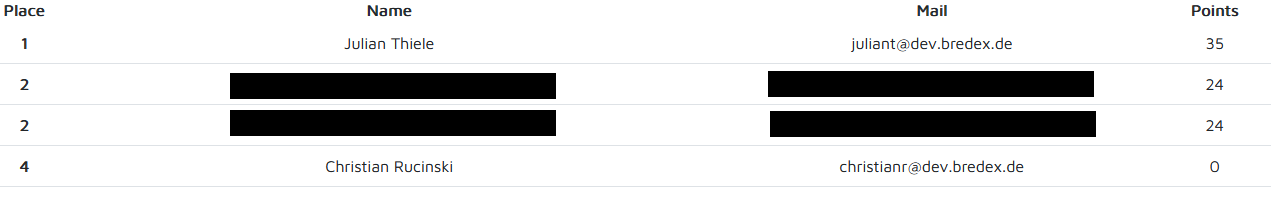
\includegraphics[width=\textwidth]{application/ranking_table.png}
    \caption{Ranking}
    \label{abb:ranking}
\end{figure}

\begin{figure}
    \centering
    
\includegraphics{application/achievement_manage.png}
    \caption{Achievements - Manage-View}
    \label{abb:achievements_manage}
\end{figure}

\begin{figure}
    \centering
    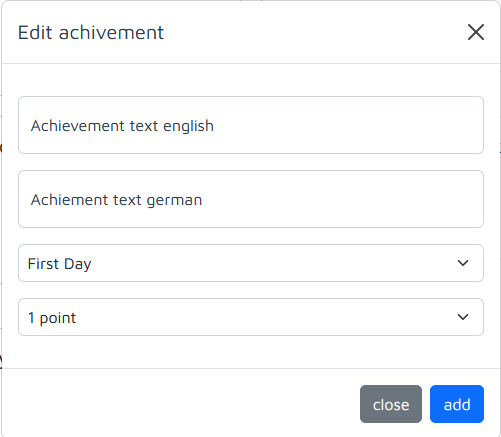
\includegraphics{application/popup_manage.png}
    \caption{Modaldialog - Add/Edit}
    \label{abb:modal}
\end{figure}

\begin{figure} % --> split in subsections
    \centering
    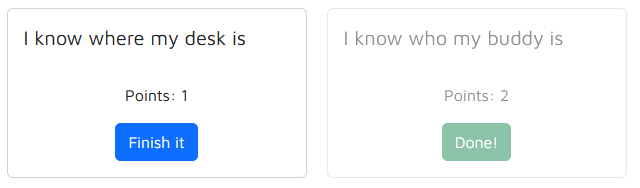
\includegraphics[width=\textwidth]{application/achievement_done_undone.png}
    \caption{Achievements}
    \label{abb:achievements}
\end{figure}

\clearpage
%----------------------------------------------------------------------------------
%----------------------------------------------------------------------------------

\begin{lstlisting}[language=TypeScript, caption=Lade Daten Beispiel]
fetchData() {
    firebase.firestore().collection("/achievements")
        .onSnapshot(snapshot => {
            this.achievements = []
            snapshot.forEach(doc => {
                this.achievements.push({
                    id: doc.id,
                    name_de: doc.data().name_de,
                    name_en: doc.data().name_en,
                    timestamp: doc.data().unlock_time,
                    points: doc.data().points
                })
            })
        })
}
\end{lstlisting}

\begin{lstlisting}[language=TypeScript, caption=OnMounted-Lifecyclehook Beispiel]
OnMounted(async () => {
    doneTasks.value = UserService.getDoneAchievements();
})
\end{lstlisting}

\begin{lstlisting}[language=Typescript, caption=Achievement Datenmodell]
{
    id: string,
    data: {
        name_de: string,
        name_en: string,
        points: int,
        unlock_time: int,
    }
}    
\end{lstlisting}

\clearpage

% use of ref
% router access management

\appendix

\section{genutzte Ressourcen}
\textbf{Personal}
\begin{itemize}
    \item Projektbetreuer
    \item Prüfungsteilnehmer
\end{itemize}
\textbf{Software}
\begin{itemize}
    \item Windows 10 Professional
    \item VisualStudio Code
    \item \Gls{firebase} als \gls{baas}
    \item \Gls{firestore} als Datenbank
    \item \Gls{git}
    \item GitLab
    \item GitHub
\end{itemize}
\textbf{Hardware}
\begin{itemize}
    \item ThinkPad
    \item 2 Monitore
    \item Tastatur
    \item Maus
\end{itemize}
\newpage
\phantomsection\addcontentsline{toc}{section}{Benutzerdokumentation}

\includepdf[pages=-]{./benutzerdoku/userdoku.pdf}
\phantomsection\addcontentsline{toc}{section}{Projektantrag}

\includepdf[pages=-]{./pictures/Projektantrag.pdf}
\phantomsection\addcontentsline{toc}{section}{Bestätigung über die durchgeführte Projektarbeit}
\includepdf[pages=-]{./pictures/Bestätigung.pdf}

% Bestätigung

\end{document}